\section{Exercises on Minimum Spanning Trees Problems}

\paragraph{}
\begin{quote}
	GTC has been provided with 50 locations to connect in a certain country. These locations need
to be connected in such a way that any two of these locations are able to communicate
with each other. All the connections need not be direct. Due to high bandwidth
requirements, GTC will use high capacity cables for the connections, and wants to
know the costs of laying the cable under various circumstances. In Figure \ref{graph2-1} we
have schematically depicted the 50 locations and all possible direct connections. The
numbers attached to the connections in Figure \ref{graph2-1} refer to the distances (in 10 kilometer
units) between locations. The cost of the cable is \texteuro 5,000 per kilometer.
\end{quote}

\begin{figure}[H]
	\centering
	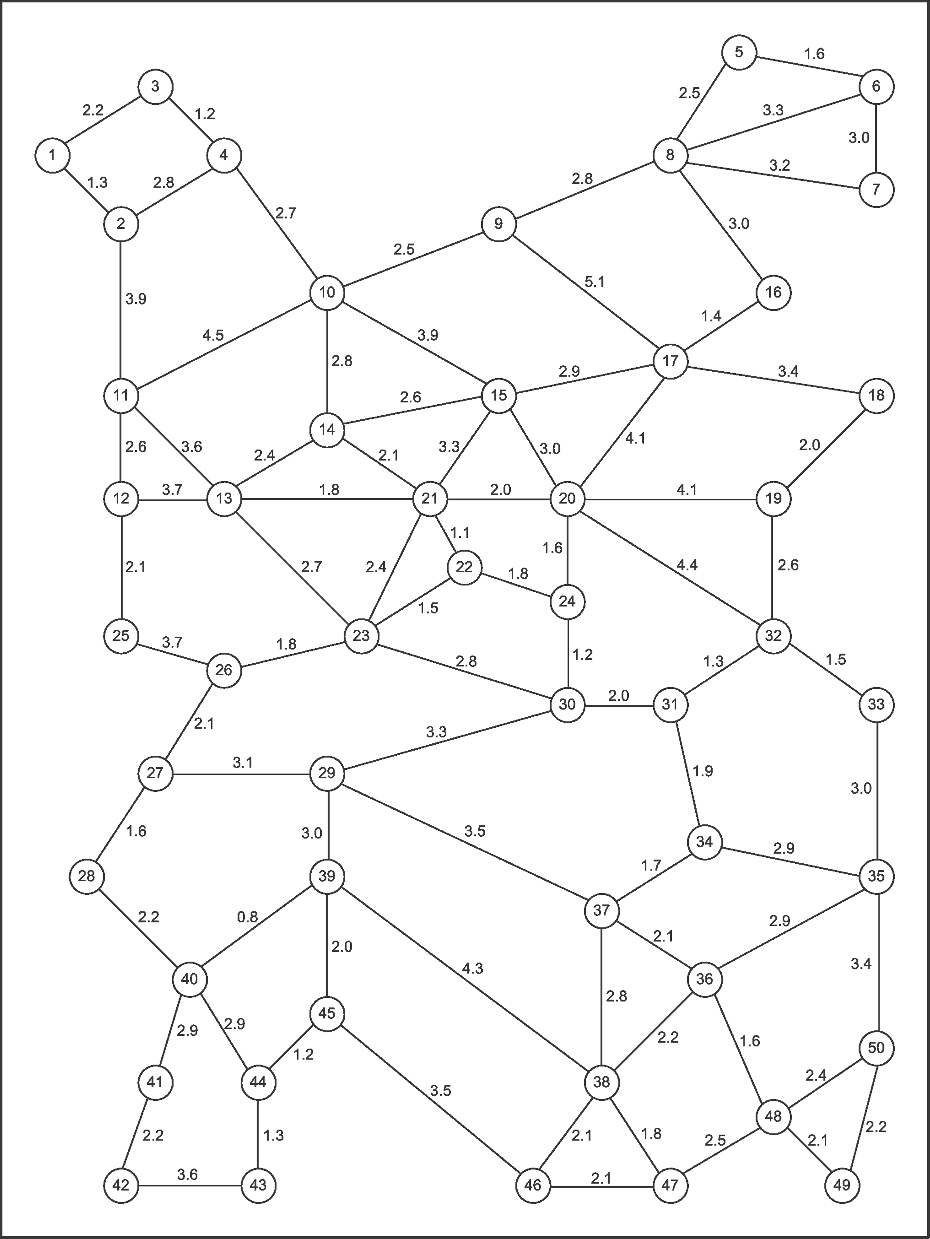
\includegraphics[scale=0.5]{./img/graph2-1.png}
	\caption{Schematic map with 50 locations (distances in 10 kilometer units, costs in \texteuro5,000per kilometer)}
	\label{graph2-1}
\end{figure}

\subsection{Problem 2.1. Reliable Cable Connections}
\begin{enumerate}[(a)]
\item \begin{quote}Calculate the minimum length of cable needed to connect all locations in Figure
\ref{graph2-1}. Also give the list of connections that are used for the cabling.\end{quote}
\end{enumerate}

\paragraph{}
	Let's consider a graph with vertices corresponding to the locations in a country and edges corresponding to possible direct connections. This graph is undirected because the cable connections transmit data in both directions and weighted --- weight of a particular edge connecting two vertices is a length of a possible direct connection in km between two corresponding locations.

\paragraph{}
	Then the sought for system of connections between locations with a minimum length of cable required is a minimum spanning tree in a described graph. Indeed in the spanning tree there is a unique path between each pair of vertices so there are no redundant connections and every location is able to communicate with other locations using cables of this system. Also by definition the sum of weights of edges in a MST is minimal possible among all the spanning trees of the graph so this system requires the minimal possible length of cable to connect all the location thus the minimal possible sum of money because we pay equally \texteuro 5,000 for every km.

\paragraph{}
	MST problem can be solved efficiently using Kruskal's algorithm. The edges of the MST (the connections between locations in the country) are listed in the figure \ref{mst1}. The length of cable needed to connect all locations is 1000 km which results in a \texteuro 5,000,000 total price of the system.

\begin{figure}[H]
	\centering
	\begin{multicols}{5}
(1,~2), (1,~3), (3,~4), (4,~10), (5,~6), (5,~8), (6,~7), (8,~9), (9,~10), (10,~14), (11,~12), (11,~13), (12,~25), (13,~21), (14,~15), (14,~21), (15,~17), (16,~17), (18,~19), (19,~32), (20,~24), (21,~22), (22,~23), (22,~24), (23,~26), (24,~30), (26,~27), (27,~28), (28,~40), (29,~39), (30,~31), (31,~32), (31,~34), (32,~33), (34,~35), (34,~37), (36,~37), (36,~38), (36,~48), (38,~46), (38,~47), (39,~40), (39,~45), (40,~41), (41,~42), (43,~44), (44,~45), (48,~49), (49,~50)
	\end{multicols}
	\caption{List of connections in a minimum cost communication system}
	\label{mst1}
\end{figure}